\documentclass[11pt,oneside]{article}
\usepackage[utf8]{inputenc}
\usepackage[T1]{fontenc}
\usepackage[british]{babel}
\usepackage{graphicx}
\usepackage[dvipsnames]{xcolor}
\usepackage[sb]{libertine}
\usepackage[scale=0.9]{inconsolata}

\usepackage[sf]{titlesec}
\usepackage{float}
\usepackage[square,sort,colon,authoryear]{natbib}
\usepackage{graphicx}
%\usepackage[export]{adjustbox}

\usepackage{
  marginnote, % Improved margin notes
  environ,
  ragged2e,   % Justified text in the margin notes
  url,        % For typesetting URLs
  listings,   % Code formatting
  lipsum,
  booktabs,
  changepage,
  float,
  dingbat
}
\renewcommand{\bfdefault}{bx}
\DeclareTextFontCommand\textsb{\libertineSB}

\usepackage[hidelinks]{hyperref}
\usepackage[capitalise]{cleveref}
\Crefname{section}{\S}{\S\S}

\usepackage{enumitem}   % Improved lists 
% \setlist{noitemsep} % To make all lists compact
\setlist[itemize]{itemsep=0pt}
\setlist[itemize,1]{label=--}
\setlist[itemize,2]{label=\ensuremath{\triangleright}}
\setlist[itemize,3]{label=\RED{AVOID}}
% Description lists to use semibold labels
\setlist[description]{font=\libertineSB}

\usepackage[oneside,labelfont=sf]{caption}

\captionsetup{justification=raggedright,singlelinecheck=false}

\newcommand\myhrulefill[1]{\leavevmode\leaders\hrule height#1\hfill\kern0pt}
\DeclareCaptionFormat{FigFormat}{{\color{black}\myhrulefill{0.5pt}}\\#1#2#3}
\captionsetup[figure]{format=FigFormat}
\captionsetup[table]{format=FigFormat}

\DeclareCaptionFormat{LstFormat}{\textsf{Listing}~\arabic{section}.\arabic{listing}:#2#3}
\floatstyle{ruled}
\newfloat{listing}{thp}{lol}[section]
\floatname{listing}{Listing}
\captionsetup[listing]{format=LstFormat}

\NewEnviron{MarginNote}[1][0mm]{\marginnote{\footnotesize\justifying\BODY}[#1]}
\newcommand{\Footnote}[2][0mm]{\footnotemark\marginnote{\footnotesize$^{\arabic{footnote})}$~#2}[#1]}

\renewenvironment{figure*}[1][]{%
  \begin{figure}[#1]%
	% This feature is deprecated for now
	% \checkoddpage%
	% \ifoddpage%
	%   \begin{adjustwidth}{0cm}{-45mm}%%
	% \else%
	%   \begin{adjustwidth}{-45mm}{0cm}%%
	% \fi%
	}{%
	% \end{adjustwidth}%
  \end{figure}}

\renewenvironment{table*}[1][]{%
  \begin{table}[#1]%
	% This feature is deprecated for now
	% \checkoddpage%
	% \ifoddpage%
	%   \begin{adjustwidth}{0cm}{-45mm}%%
	% \else%
	%   \begin{adjustwidth}{-45mm}{0cm}%%
	% \fi%
	}{%
	% \end{adjustwidth}%
  \end{table}}

\renewenvironment{listing*}[1][]{%
  \begin{listing}[#1]%
	% This feature is deprecated for now
	% \checkoddpage%
	% \ifoddpage%
	%   \begin{adjustwidth}{0cm}{-45mm}%%
	% \else%
	%   \begin{adjustwidth}{-45mm}{0cm}%%
	% \fi%
	}{%
	% \end{adjustwidth}%
  \end{listing}}

%% == Code =======================================================
\lstnewenvironment{Code}[1][style=std]{\lstset{#1}}{}
\lstnewenvironment{Code_Numbered}[1][style=std,numbers=left]{\lstset{#1}}{}

\renewcommand{\c}[1]{\lstinline[style=std]@#1@}

\lstdefinestyle{std}{
  language=java,
  basicstyle=\small\tt\color{black},
  keywordstyle=\small\tt\bfseries,
  numberstyle=\footnotesize\sf\color{black},
  commentstyle=\small\color{black}\it,
  aboveskip=1ex,
  belowskip=1ex,
  tabsize=2,
  columns=fullflexible,
  xleftmargin=1ex,
  resetmargins=true,
  showstringspaces=false,
  morecomment=[l]{//},
  morecomment=[l]{--},
  morecomment=[s]{/*}{*/},
  escapeinside=@@,
  morekeywords={Frobies},
  moredelim=[is][\textit]{___}{___},
  moredelim=[is][\textbf]{__*}{*__},
  numberbychapter=true
}

\usepackage[activate={true,nocompatibility},final,tracking=true,kerning=true,spacing=true,factor=1100,stretch=10,shrink=10]{microtype}
\usepackage[paper=a4paper,text={13cm,24cm},marginparsep=5mm,marginparwidth=45mm,inner=20mm]{geometry}

\newcommand{\RED}[1]{\textcolor{red}{#1}}
\newcommand{\ie}{\emph{i.e.,}}
\newcommand{\eg}{\emph{e.g.,}}
\newcommand{\etal}{\emph{et~al.}}

\usepackage{pifont}
\newcommand{\Yes}{\ding{51}}
\newcommand{\No}{\ding{55}}

\renewcommand{\bfdefault}{b}
\clearpage

%% You can remove this line if you compile with --synctex=1 (see Makefile)
\synctex=1
\pagestyle{plain}

\begin{document}

\begin{titlepage}
    \centering
    \vspace*{3cm} % Pushes content down the page

    {\Huge\bfseries Group 15 Project Report\par}
    \vspace{2cm}

    {\Large Adnan Erlangga Raharja, Ha Pham, Yasiru Bhagya, Yoav Kalisher\par}
    \vspace{2cm}

    {\Large \today\par}

    \vfill
\end{titlepage}

\vspace*{3cm}

\section*{Abstract}
\addcontentsline{toc}{section}{Abstract}

Today, students in higher education must manage a wide variety of tasks in very constrained timeframes as a part of their studies, which necessitates the use of tools to better manage their workload. Prior research has shown that poor time management and academic stress can significantly affect student performance and well-being \citep{misra2000college}; likewise, effective learning strategies and self-regulation are key predictors of academic success \citep{zimmerman2002becoming}.

However, despite how many of these tools exist, very few of them are tailored for students. Our team hopes to create a free tool that can fill this gap. We aim to create a web-based task management tool that provides students with the ability to manage both their individual work and work they need to do in groups. The tool should be able to run on any computer to fit a variety of different use cases, from cloud-based servers to students' personal computers. We also aimed to make the tool accessible for students with a wide variety of different backgrounds.

Through our efforts, we were successful in creating a flexible and portable task management tool. The tool can run on systems with even minimal computing power and works for a variety of different tasks. However, there is still room for improvement to add more functionality and improve accessibility with better language and task input support.

\clearpage
\tableofcontents
\clearpage

\section{Introduction}

Task management systems are usually used by the project development teams to track their tasks from beginning to end, delegate subtasks to teammates, and set deadlines to make sure projects get done on time \citep{nurzi2022web}. While these systems are traditionally associated with professional project development teams, the same concept is now increasingly applied in educational contexts. Studies highlight that higher education students often face cognitive overload when balancing multiple courses and activities \citep{kirschner2013learners}. 

Today, students in higher education must manage a wide variety of tasks in very constrained timeframes as a part of their studies, from individual homework assignments and readings to group projects and preparation for exams. This workload necessitates tools that enable students to organize and prioritize their work to be successful. Because of how ubiquitous computer technology is today, there are a large number of tools that leverage the internet to allow for easy access from most consumer computer devices. Some of the most common and well-known task management applications, widely used by professionals, are Trello \citep{shchetynina2022trello}, Todoist \citep{bourbon2021time}, and Notion \citep{reach2022notion}, as they combine ease of use with features such as visual organization, reminders, and flexible customization.

However, despite how many of these tools exist, very few of them are tailored for students. Many of them are designed either for large corporate teams or for individuals with very simple needs, neither of which work well for the in-between needs that students have. Task managers that are more fitting for students are often prohibitively expensive for them, as they require yearly subscriptions and most students don’t have a consistent expendable income. As a result, there aren’t many good options for students. This is especially true when it comes to managing group work for classes, something that is particularly relevant when studying at a Swedish university where it is very common to have classes that primarily consist of group work.

\section{Background}
\label{cha:background}
\subsection{Current Options for Task Managers}
A wide variety of internet-based task management tools currently exist. These are offered by a wide variety of companies, some of which specialize in creating these tools while others provide them as a part of a larger suite of tools.

Google, Microsoft, and Apple, companies with a major web presence and billions of active user accounts, all provide simple task managers as a part of their free accounts that are accessible from any device with a web browser. These tend to have limited functionality, allowing for the creation of simple tasks containing a title and a due date. Microsoft’s and Apple’s task managers also allow for collaboration with more than one person, but both require that all users have an account with them. Despite these companies’ wide reach, it is common for individuals to only have active accounts with one or neither of these two companies. In Apple’s case in particular, the company’s Reminders app is only available on Apple’s platforms, further shrinking the availability of the tool.


Other companies, such as Doist, Inc., the Omni Group, and Cultured Code provide more complex and feature-rich applications, but their products all require costly purchases or subscriptions. Furthermore, of these three companies, only Doist offers a task manager that allows for collaboration, but this application is also the most expensive of the three.

Finally, Atlassian and Asana create tools that are specifically designed for working in teams. However, these tools are specially designed for specific workflows in corporate teams, and are inflexible and difficult to use in other settings. Group work in higher education has been widely recognized as both a pedagogical opportunity and a source of coordination challenges \citep{johnson2009educational}; studies emphasize that collaborative learning, while beneficial, requires effective task organization and communication tools \citep{dunlosky2013improving}.

We have also explored the efficacy of leveraging free general-purpose note taking tools, such as Google docs, as task management tools in groups. While this was technically possible, it was unwieldy and difficult to manage, as tasks could easily get lost in large projects and having multiple team members creating and updating tasks at once made the document difficult to track in real time, leading to both redundancy and missing tasks.
\subsection{Types of Student Tasks}
Students have four key types of tasks that we have identified as a part of their studies: 

\begin{enumerate}
\item Individual homework assignments – These entail work that each student does by him- or herself, often consisting of multiple parts to complete. For example, a student may have to submit a C programming assignment that has to enable a specific set of functionality, or a student may have to write an essay about a topic with a specific structure. These often have strict deadlines, either for individual components or for the submission as a whole.
\item Self-guided learning – Many classes require students to do additional self-guided learning outside of lectures in the form of articles and books to read or videos to watch. These vary in length, content, and structure, but can usually be broken down into discrete subparts. Most teachers do not have formal deadlines for the learning, but will reference it throughout the course or will expect the student to use the knowledge in various assignments or exams.
\item Exam preparation – Many courses end with a comprehensive exam covering all of the material taught in the course. Evidence shows that some study techniques are much more effective than others \citep{dunlosky2013improving}, which reinforces the importance of structured preparation tools. Succeeding in these exams requires extensive preparation and review of the course’s provided resources, and may also entail completing practice exams or exercises provided by the instructor.
\item Group work – Group work is similar to individual work, with the added complexity of having to communicate and orchestrate tasks with other students. This means all members of the group should have easy access to not just which tasks need to be done for an assignment, but also the current state of all tasks and who is assigned to work on them. This also includes needing to be able to schedule times when work needs to be done in teams.
\end{enumerate}



\section{Methodology}
\subsection{Scope}
We determined the functional requirements for our task management tool based on our own experiences as students getting master’s degrees from Uppsala University. Of our four group members, two of us are majoring in computer science, and two are majoring in embedded systems. We used our current courses for reference on the kind of tasks we would need to be able to track in the application, and compared them to the tools we currently have access to. 

Furthermore, we scoped the project based on specific constraints provided by the course. We had 8 weeks to design, implement, test, and deploy our project, and needed to utilize a raspberry pi in the process. Our team also primarily had experience writing backend applications in python and simple frontend applications with javascript, HTML, and CSS. As a result, we determined the most effective way for us to build this application was to create a python-based REST API [14] that could be hosted on a raspberry pi, and would have a simple web frontend that would make requests to the backend to view, edit, and manage tasks.

We began with a list of base requirements that our tool needed to be able to handle. The tool needed to allow for users to create accounts to store their task data. Both the frontend and backend needed to be able to handle logins, sessions, and invalid login attempts. Then, the frontend needed to be able to show a list of tasks and give the user the ability to add, edit, delete or mark tasks as complete. Likewise, the backend needed to have endpoints to enable each of those functions for a specified user for a specified task. These functions needed to be clear and doable from both desktop and mobile browsers.

Additionally, we wanted to add “chatbot” functionality to add tasks via natural language. On the frontend, this meant adding an interface that allowed users to type in tasks they wanted to add with the details they cared about. On the backend, we created an additional endpoint to parse the user’s request using a structured format, and then making additional requests to the relevant endpoints. The backend also needed to handle requests that weren’t structured properly, and respond with appropriate messages to explain to the user how to make a correct request. 

\subsection{Workflow}
Our team used a waterfall-style model of software development. We began by defining the scope and requirements of the app and what functionality we expected to implement when. Then we split up the work into different roles and assigned roles to each team member. We identified four core roles:

\begin{enumerate}
\item Project Manager - In charge of managing communication, ensuring project is on track or providing support to keep project on track, and documenting progress.
\item Frontend Developer - In charge of creating interactive user interface for the app
\item Backend Deveoper - In charge of creating the API and database for the app
\item QA Engineer - In charge of testing and validating the app, ensuring the product meets requirements, and documenting outcomes.
\end{enumerate}

The team met every week virtually to discuss progress, blockers, and upcoming deadlines, and maintained active communication through Whatsapp to coordinate tasks that required multiple team members. All of our code was stored on a shared github repository that we all had access to, ensuring we could test new features and provide feedback.

\section{Ethical Considerations}
Students have a wide variety of backgrounds and needs when it comes to creating and managing tasks. Prior work emphasizes that digital learning and productivity tools must take into account diverse accessibility requirements to avoid excluding certain groups of learners \citep{seale2013learning}. We wanted to be mindful of this when designing our website by ensuring that it is accessible for a wide variety of people. This meant providing features like the ability to change text to more dyslexic-friendly fonts or to be larger, ensuring there was enough space for users to enter tasks in different languages \citep{al2016universal}, and providing options for how much information a user wants to see at once in case they may feel overwhelmed seeing too many tasks at once \citep{spina2019wcag}. International perspectives on accessibility stress that tools should be adaptable to diverse cultural and linguistic contexts \citep{world2011world}.

We also wanted to ensure our app was available to as many students as possible, as one of the primary issues with existing tools is that their cost or functionality made them inaccessible to many students. Studies have noted that cost and resource constraints are significant barriers to equitable access in higher education technology \citep{selwyn2021education}. This is why we made our web app freely available and able to be hosted using freely available tools. We also ensured the app was efficient and could run on low-end computer hardware, which aligns with research emphasizing the importance of universal design and low-barrier entry points \citep{rose2002teaching}. Other work on inclusive HCI methods highlights the importance of testing accessibility features systematically \citep{lazar2017research}.

One of our last big accessibility features was to make the tool more accessible by allowing users to add tasks via natural language.  Natural language interfaces have been shown to improve usability for users with varying levels of technical proficiency \citep{shneiderman2010designing}, and they can make interaction with digital tools more intuitive for students unfamiliar with structured task management systems. Similar findings are reported in educational technology studies, where natural language input has been linked to improved engagement \citep{junco2012relationship}.


\section{Implementation}

Our web app was split into two parts: the backend, which would run on our raspberry pi and run our API and database, and the frontend, which handled user interactions on a browser. We also had a telegram bot that could be used to enter tasks using structured language.

\subsection{Backend}
Our backend consisted of an API and a database. Our API was written in python using the Flask framework, and had endpoints for authentication and managing task data. We had the following endpoints available:

\begin{table}[H]
    \centering
    \caption{Backend API Endpoints}
    \label{tab:api-endpoints}
    \begin{tabular}{l l p{8cm}}
        \toprule
        \textbf{HTTP Method} & \textbf{Endpoint} & \textbf{Description} \\
        \midrule
        POST & /api/auth/register & Register a new user. \\
        POST & /api/auth/login & Login user and get access token. \\
        GET & /api/auth/me & Get current user info (requires authentication). \\
        DELETE & /api/auth/delete-account & Delete account and all user's tasks (requires authentication). \\
        GET & /api/tasks & Get current user's tasks (supports filtering). \\
        POST & /api/tasks & Create a new task for current user. \\
        GET & /api/tasks/\textless id\textgreater & Get a specific task (if owned by current user). \\
        PUT & /api/tasks/\textless id\textgreater & Update a specific task (if owned by current user). \\
        DELETE & /api/tasks/\textless id\textgreater & Delete a specific task (if owned by current user). \\
        \bottomrule
    \end{tabular}
\end{table}

These endpoints met the privacy requirements of our system, ensuring users only have access to their own tasks, and the functional requirements of our system, ensuring users could flexibly manage their tasks.

Our database had two main tables: users and tasks. Our user table was simple: a name, email, password, and internal ID. Our task table was larger, and included more information.

\begin{table}[H]
    \centering
    \caption{Database Schema for Task Table}
    \label{tab:database-schema}
    \begin{tabular}{l l p{8cm}}
        \toprule
        \textbf{Field} & \textbf{Type} & \textbf{Description} \\
        \midrule
        Title & string & User-provided title for the task. \\
        Description & string & User-provided description for the task. \\
        Priority & string & Defined as a string in the database. \\
        User ID & UUID & Owning user. \\
        Due date & date & Due date of the task. \\
        Status & string & User-provided status of the task (e.g., \texttt{todo}, \texttt{finished}, etc.). \\
        \bottomrule
    \end{tabular}
\end{table}

The task endpoints would be used to interface with the database in order to avoid users directly manipulating data and accidentally causing errors.

\subsection{Frontend}

\begin{figure}[H]
    \centering
    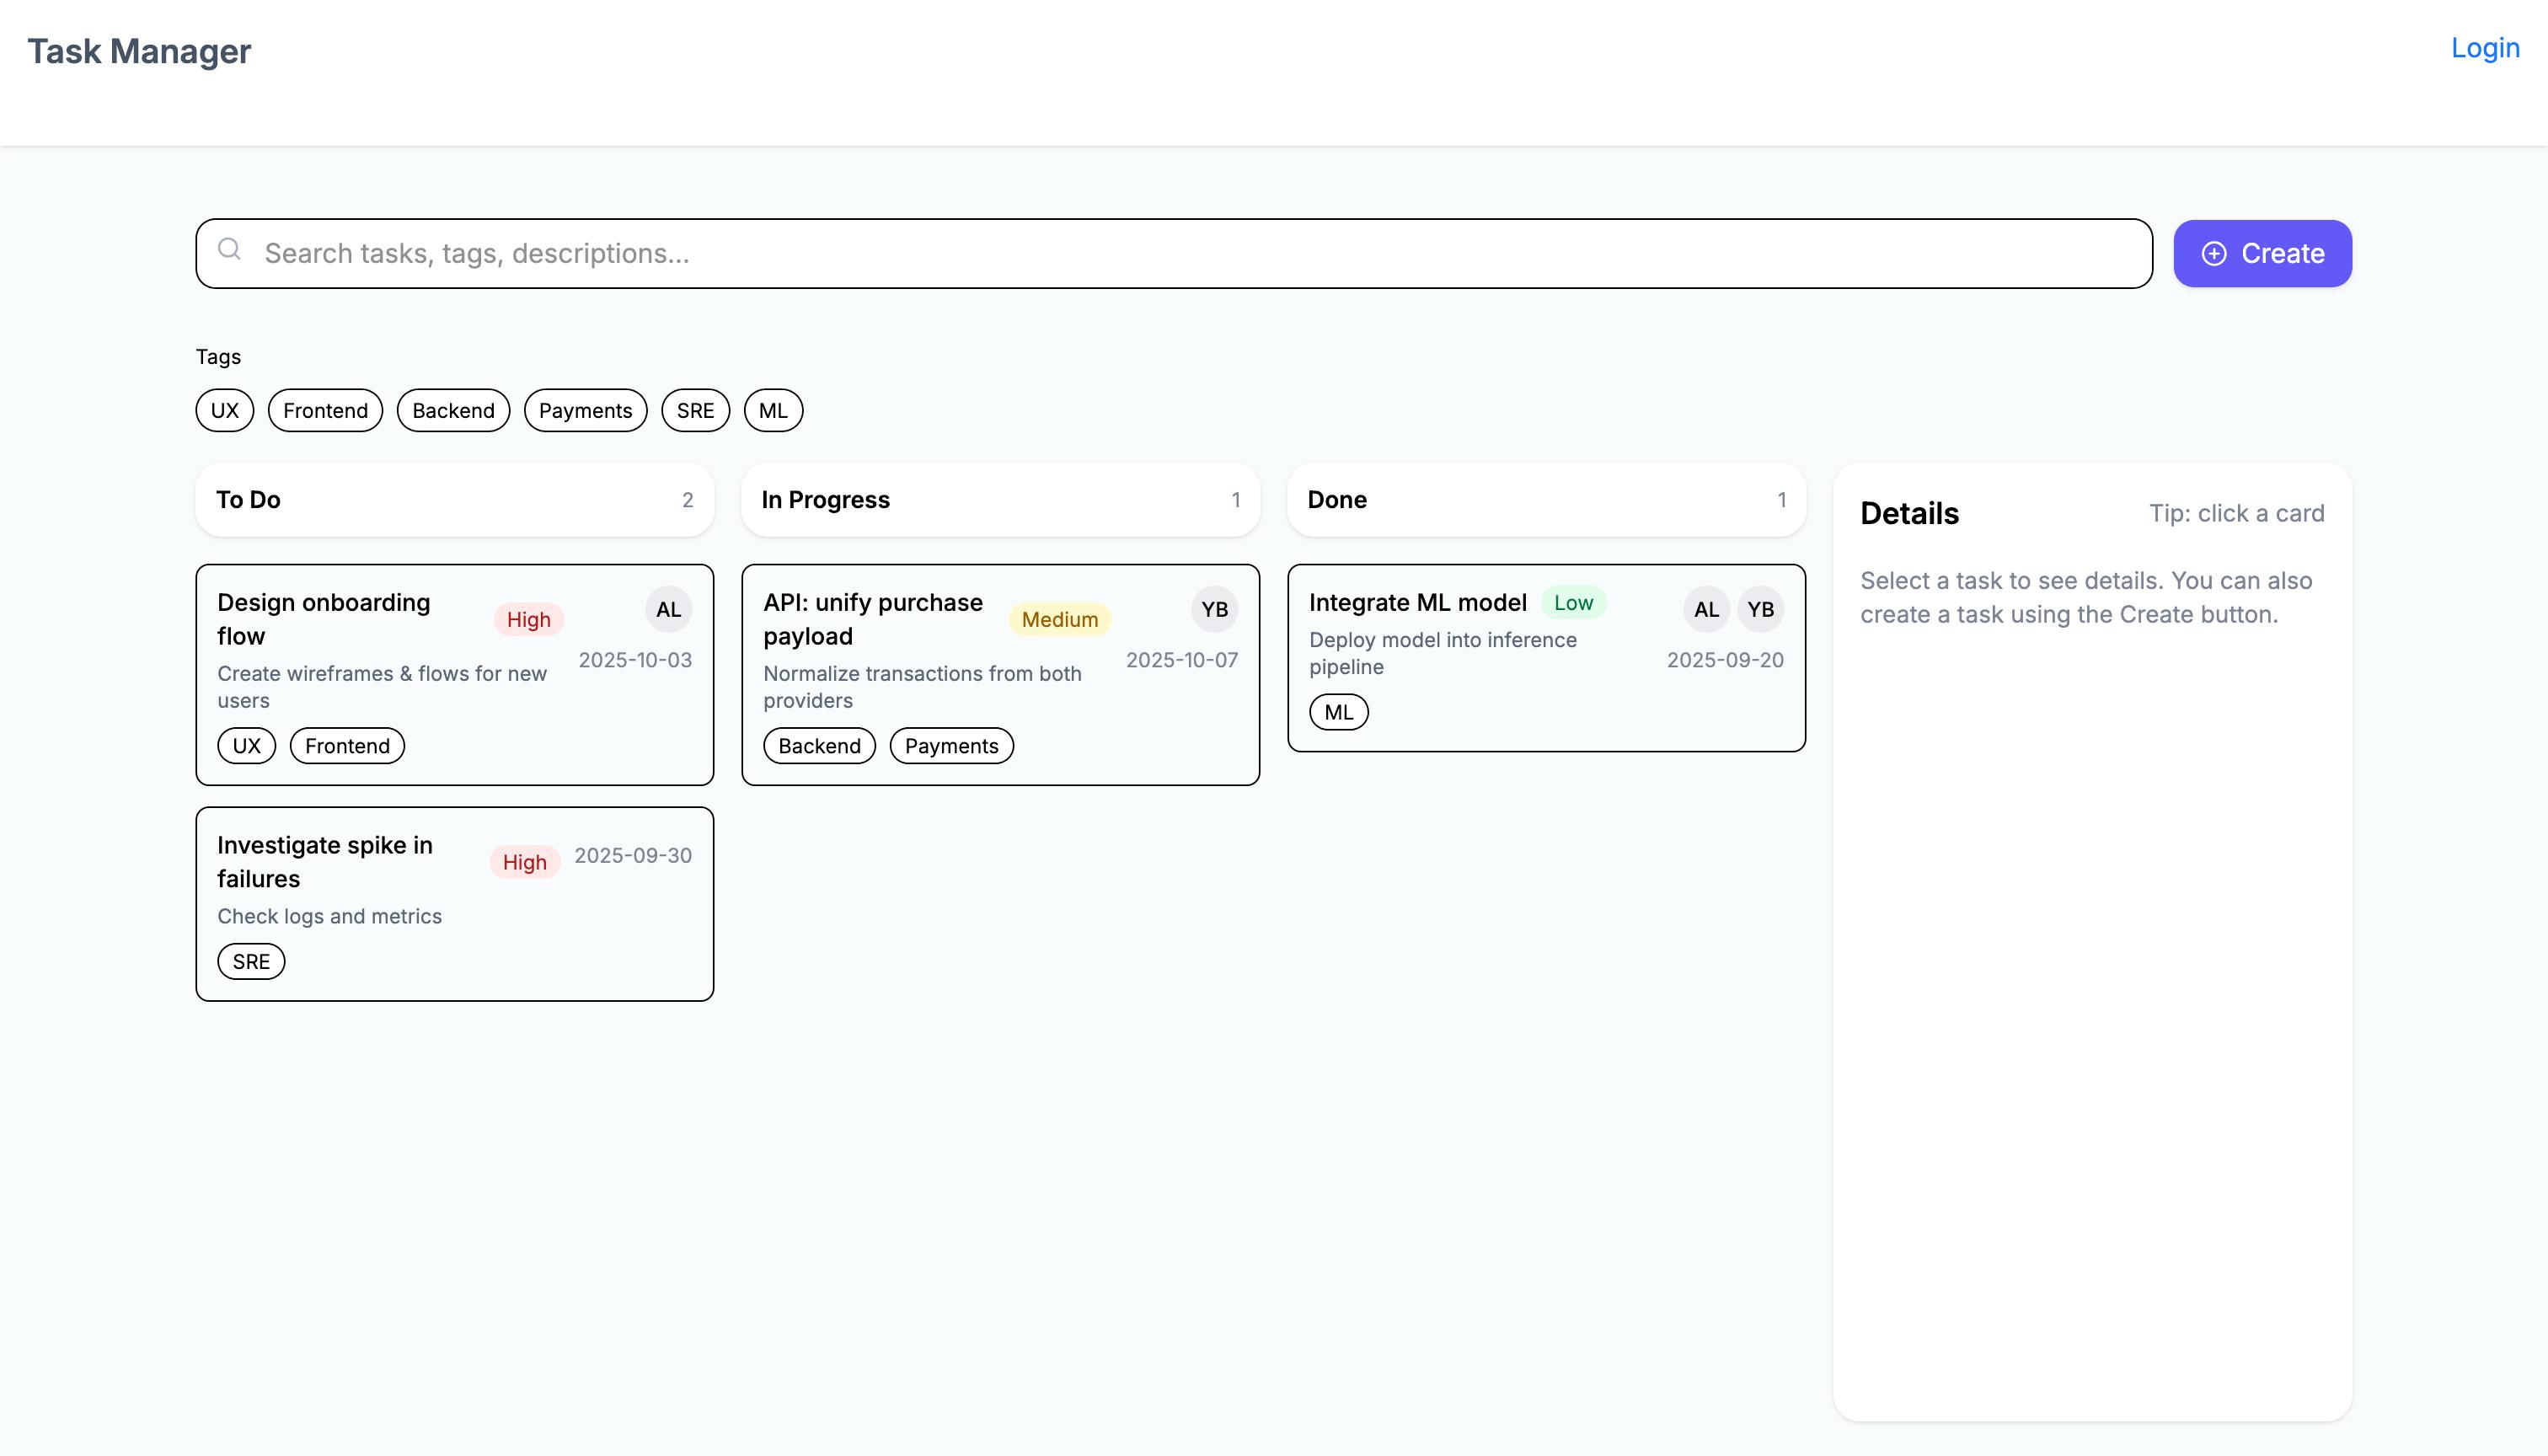
\includegraphics[width=1.0\textwidth]{dashboard_screenshot.jpeg}
    \caption{Screenshot of the Dashboard with Example Tasks}
    \label{fig:dashboard-screenshot}
\end{figure}

Our frontend has a few different pages to enable the user to use our task manager. We have a few pages for user management (logins and registration) but most of the work went into the main task dashboard.

The dashboard is where users can add, edit, and interact with tasks. All tasks are clickable and editable from this page. Task data can be edited as text where relevant (for title and description, for example), and the user can also drag tasks between different subsections.

We decided to structure the dashboard as a kanban board because it fit neatly with having a status, and provides an easy interface for quickly identified what has to be done and when.

Along with all of the core pieces mentioned earlier, the frontend also adds the ability to add tags to tasks. Each task can be assigned multiple tags, and multiple tasks can have the same tag. The user can then filter on the dashboard to only see tasks with specified tags, which allows the user to focus on a specific project or area instead of having to see everything at the same time.

Unfortunately, we did not have time to add functionality so that multiple different users could see the same task. While this was an important part of our project, we did not have the time to build a secure version of the feature, and the feature had to be dropped.

\subsection{Telegram Bot}

\begin{figure}[H]
    \centering
    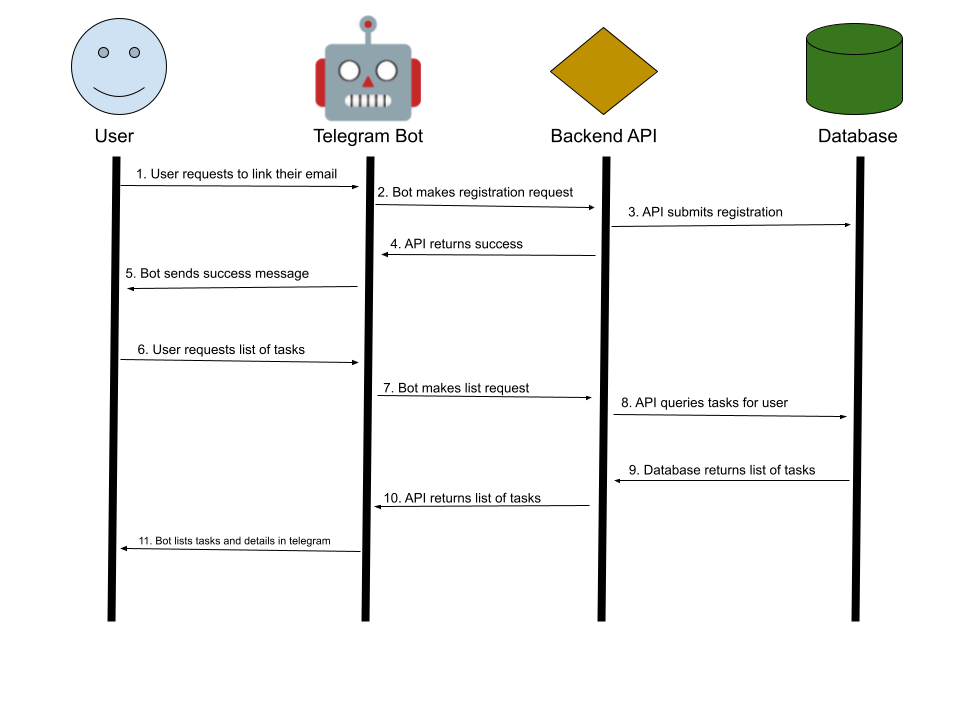
\includegraphics[width=1.0\textwidth]{telegram_bot.png}
    \caption{Sequence Diagram of Telegram Bot Interactions}
    \label{fig:telegram-diagram}
\end{figure}

\begin{figure}[H]
    \centering
    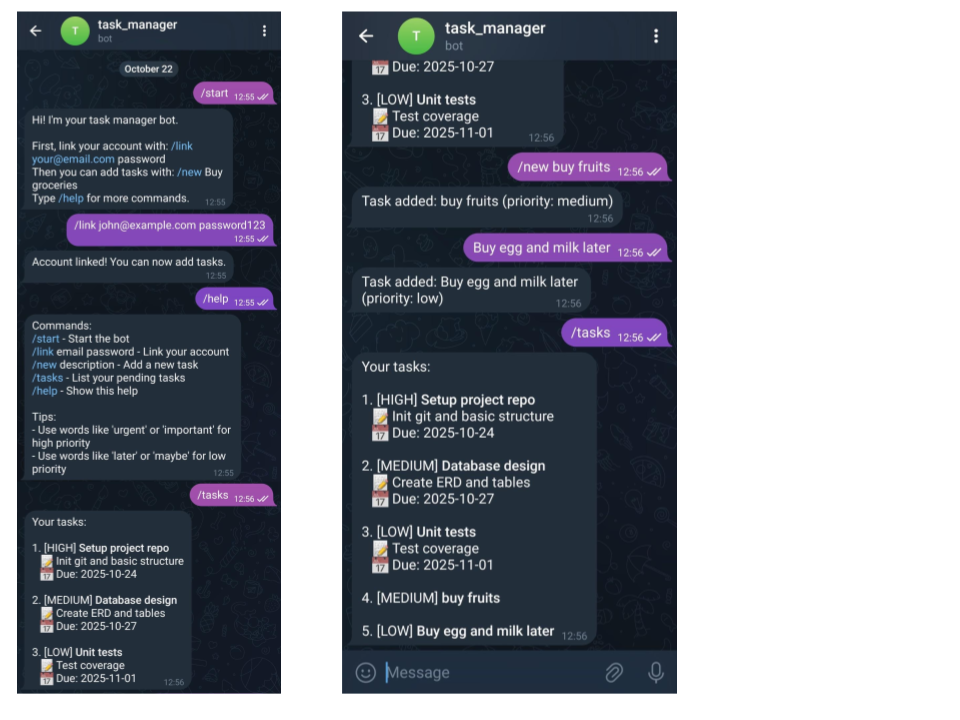
\includegraphics[width=0.8\textwidth]{telegram_example.png}
    \caption{Using our Telegram bot to register and view tasks (left) and add new tasks (right)}
    \label{fig:telegram-example}
\end{figure}

Our telegram bot enables users to send structured language messages to add tasks to their database. They first have to connect their email to an account, then have access to use the bot. The bot can authorize the user, add a task, and list their current tasks. It does so by accessing the corresponding endpoints in the backend.

\section{Reflection}
Our team has gained hands-on experience with both the technical and organizational aspects of developing a web-based application when working with this project. With everything we did, our primary takeaway was the importance of matching the limited timeframe and resources available. Working on a full project in 8 weeks while juggling other responsibilities proved to be a meaningful challenge and required us to maximize all of the time we spent working. As a part of this, we also recognized trying to include too many features would have compromised stability given how little time we had to fully implement everything. From this course project, our team also learned how essential accessibility considerations are in making sure that a tool can be used by students. As we mentioned, there are a wide variety of different students with different preferences for working, and ensuring we could accomodate all of those needs required extensive consideration. Finally, this project highlighted the value of collaboration within team members: dividing responsibilities, and communicating effectively. 

In the future, the app could be improved with additional features that we did not have time to implement. Enabling group work and shared tasks would be the highest priority, followed by extensive testing and support for multiple languages and different fonts to make the tool more accessible for more users.


\section{Contributions}
Yoav and Ha co-wrote the abstract, introduction, background, methods, and ethical considerations. Methods were compiled based on notes written by each team member. Ha compiled and structured the references. Yasiru and Adnan wrote the implementation section.


\bibliographystyle{plainnat}
\bibliography{references}


\end{document}

%%% Local Variables: ***
%%% mode: latex ***
%%% TeX-master: "main.tex"  ***
%%% ispell-local-dictionary: "british"  ***
%%% End: ***